\section{Evaluation}
\label{sec:evaluation}

We evaluate four questions: \textbf{RQ1} whether the detector generalizes to
source-disjoint Skills; \textbf{RQ2} whether structured static evidence helps
beyond rules or direct document classification; \textbf{RQ3} what behavior the
graph actually recovers; and \textbf{RQ4} whether the pipeline fails safely and
scales to a current, unlabeled corpus. \textbf{Ours} denotes the complete
pipeline in Section~\ref{sec:methodology}.

\subsection{Experimental Setup}

\subsubsection{Datasets}

\textbf{MalSkillsBench-200.} We retain a fixed snapshot of the public
100-malicious/100-benign benchmark released with
MalSkills~\cite{wang2026malskills}, only as a diagnostic set.
Its labels are completely confounded with source and owner: source alone
predicts all labels, and every one of its 78 owners is class-pure. Results on
this corpus therefore cannot establish source-independent generalization.

\textbf{MaliciousSkillBench-SD1000.} Our primary labeled evaluation samples
500 malicious and 500 benign Skills from the official source-disjoint test
split of MaliciousSkillBench~\cite{wang2026maliciousskillbench}. The sample is
balanced, integrity-checked, and preserves the released labels while excluding
label and source fields from detector input. It spans three held-out source
groups (428, 425, and 147 packages).

\textbf{Community-Skills-1000.} To test current-corpus operability, we collect
100 Skills from each of ten registry categories: data, design, development,
DevOps, documents, marketing, product, productivity, security, and testing.
Selection is deterministic, capped at five Skills per repository, and retains
only the bounded primary Skill document. This corpus has no security ground
truth; its outputs are audit candidates, not estimates of malicious prevalence.

\subsubsection{Compared Methods}

\emph{Frozen rules} applies the same instruction, object, filesystem, network,
process, concealment, privilege, persistence, and destructive-operation rules
used to generate evidence for Ours, with a fixed score threshold of five.
\emph{Direct model} sends only the bounded primary Skill document to one
schema-constrained reviewer; it receives no static findings, graph, source,
registry metadata, or label. \emph{No function view} removes the independent
high-level summary while leaving the remaining Ours pipeline unchanged.

\subsubsection{Protocol and Metrics}

Targets are streamed as data and are never installed, imported, or executed.
Each package is bounded to 128 files, 256~KiB per file, and 750,000 characters.
Model stages use \texttt{deepseek-v4-flash}, temperature zero, thinking
disabled, closed JSON schemas, and deterministic local validation. Predictions
and failures are checkpointed per sample; two bounded resume passes retry only
unresolved samples. We report coverage separately and never impute failures.

Malicious is the positive class. We report Precision, Recall, F1, FPR,
accuracy, balanced accuracy, MCC, and three-way disposition. Confidence
intervals use 1,000 class-stratified bootstrap replicates with seed 1337.
Paired comparisons use the intersection of successful samples and an exact
McNemar test.

\subsection{RQ1: Source-Disjoint Detection}

Table~\ref{tab:source-disjoint} changes the conclusion suggested by the small
benchmark. On the 977 packages shared by all methods, Ours nearly eliminates
false positives, but detects only 57/491 malicious Skills. Direct document
classification doubles recall while retaining high precision, and is correct
on 54 samples that Ours misses versus four in the opposite direction
($p=3.17\times10^{-12}$). Thus, structured evidence does not outperform a
strong direct model under source separation.

\begin{table*}[!t]
\centering
\caption{Source-disjoint results on 977 common successful packages. Counts
precede percentages; higher is better except FPR.}
\label{tab:source-disjoint}
\small
\resizebox{\textwidth}{!}{%
\begin{tabular}{lrrrrrrrr}
\toprule
Method & TP/FP/TN/FN & Precision & Recall & F1 & FPR & Accuracy & Bal. Acc. & MCC \\
\midrule
Frozen rules & 53/53/433/438 & 53/106 (50.00\%) & 53/491 (10.79\%) & 17.76\% & 53/486 (10.91\%) & 486/977 (49.74\%) & 49.94\% & $-0.002$ \\
\textbf{Ours} & \textbf{57/1/485/434} & \textbf{57/58 (98.28\%)} & \textbf{57/491 (11.61\%)} & \textbf{20.77\%} & \textbf{1/486 (0.21\%)} & \textbf{542/977 (55.48\%)} & \textbf{55.70\%} & \textbf{0.241} \\
Direct model & 109/3/483/382 & 109/112 (97.32\%) & 109/491 (22.20\%) & 36.15\% & 3/486 (0.62\%) & 592/977 (60.59\%) & 60.79\% & 0.339 \\
\bottomrule
\end{tabular}%
}
\end{table*}

Bootstrap intervals reinforce the gap: Ours reaches 11.61\% recall
[8.76\%, 14.66\%] and 20.77\% F1 [16.10\%, 25.44\%], whereas the direct model
reaches 22.20\% recall [18.74\%, 25.87\%] and 36.15\% F1 [31.40\%, 40.90\%].
The precision difference is negligible relative to the recall loss.

\noindent\textbf{Finding 1.} The source-disjoint experiment rejects an overall
detection advantage for Ours; its supported advantage is a 0.21\% FPR at the
cost of very low malicious recall.

\subsection{RQ2: What Produces the Decision?}

The source-confounded 200-package diagnostic explains why the earlier result
was misleading. Ours attains 54/55 (98.18\%) precision, 54/99 (54.55\%) recall,
and 70.13\% F1 on 197 completed packages, versus 32.47\% F1 for frozen rules.
That improvement disappears under source separation. Moreover, removing the
high-level function view slightly improves the 196-sample common subset from
70.13\% to 71.79\% F1; only two predictions change, both correcting false
negatives ($p=0.50$). The evidence therefore falsifies the intended
function--behavior consistency contribution on the available benchmark.

Ours' low binary FPR is achieved through abstention rather than benign
resolution. Figure~\ref{fig:triage} shows the source-disjoint common subset:
277/491 malicious packages are contained by \textsc{Block} or
\textsc{Review}, but 244/486 benign packages also require review. Only
241/486 benign Skills pass automatically.

\begin{figure}[!t]
  \centering
  \resizebox{0.98\columnwidth}{!}{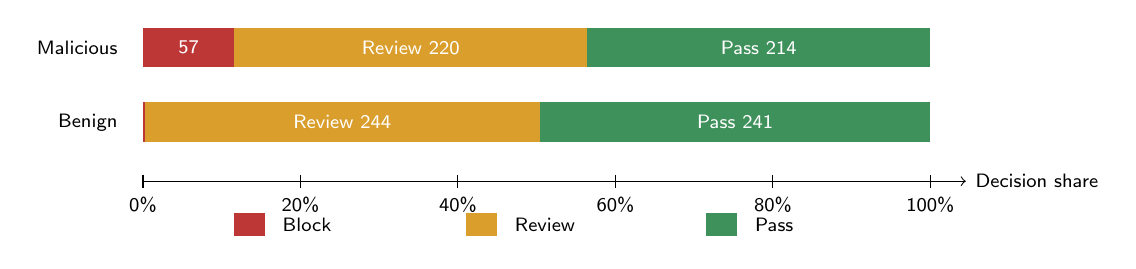
\begin{tikzpicture}[font=\sffamily\scriptsize]
  \definecolor{blockred}{RGB}{190,55,55}
  \definecolor{reviewgold}{RGB}{218,158,44}
  \definecolor{passgreen}{RGB}{63,145,92}
  \draw[->] (0,0) -- (10.45,0) node[right] {Decision share};
  \foreach \x/\lab in {0/0,2/20,4/40,6/60,8/80,10/100}
    \draw (\x,0.08) -- (\x,-0.08) node[below] {\lab\%};
  \node[anchor=east] at (-0.2,1.7) {Malicious};
  \fill[blockred] (0,1.45) rectangle (1.161,1.95);
  \fill[reviewgold] (1.161,1.45) rectangle (5.642,1.95);
  \fill[passgreen] (5.642,1.45) rectangle (10,1.95);
  \node[text=white] at (0.581,1.70) {57};
  \node[text=white] at (3.402,1.70) {Review 220};
  \node[text=white] at (7.821,1.70) {Pass 214};
  \node[anchor=east] at (-0.2,0.75) {Benign};
  \fill[blockred] (0,0.50) rectangle (0.021,1.00);
  \fill[reviewgold] (0.021,0.50) rectangle (5.041,1.00);
  \fill[passgreen] (5.041,0.50) rectangle (10,1.00);
  \node[text=white] at (2.531,0.75) {Review 244};
  \node[text=white] at (7.521,0.75) {Pass 241};
  \fill[blockred] (1.15,-0.70) rectangle (1.55,-0.40);
  \node[anchor=west] at (1.65,-0.55) {Block};
  \fill[reviewgold] (4.10,-0.70) rectangle (4.50,-0.40);
  \node[anchor=west] at (4.60,-0.55) {Review};
  \fill[passgreen] (7.15,-0.70) rectangle (7.55,-0.40);
  \node[anchor=west] at (7.65,-0.55) {Pass};
\end{tikzpicture}
}
  \caption{Ours' three-way disposition on the source-disjoint common subset.}
  \label{fig:triage}
\end{figure}

\noindent\textbf{Finding 2.} The high-level function view contributes no
measurable detection benefit, while extensive review absorbs much of the
ambiguity that would otherwise become false positives.

\subsection{RQ3: Static Graph Support}

The implementation instantiates the cross-file Python analysis described in
Section~\ref{sec:behavior}: it resolves local imports and calls, computes
parameterized summaries to a fixed point, and emits source-to-sink paths with
finite call chains. On MalSkillsBench-200, all 113 Python files parse, yielding
574 function or module bodies and 450 resolved call edges. Yet all six
source-to-sink paths occur in four benign packages; only two malicious packages
contain Python, while 206 non-Python code files lack AST-level flow support.
This benchmark therefore verifies implementation and exposes unsupported
coverage, but cannot estimate malicious-flow recall.

\noindent\textbf{Finding 3.} Cross-file graph recovery is operational, but its
security value remains unmeasured because the labeled corpus is not flow-rich
in the supported language.

\subsection{RQ4: Reliability, Cost, and Community Scale}

Table~\ref{tab:reliability} reports complete-corpus processing before the
common-subset join. Checkpointing prevents persistent structured-output errors
from terminating an experiment, but Ours completes fewer samples and uses more
than twice the recorded tokens of the direct baseline. Token totals exclude
failed requests and are therefore lower bounds.

\begin{table}[!t]
\centering
\caption{Coverage and recorded model cost on SD1000.}
\label{tab:reliability}
\small
\begin{tabular}{lrrr}
\toprule
Method & Coverage & Calls & Tokens \\
\midrule
Frozen rules & 1000/1000 (100.00\%) & 0 & 0 \\
\textbf{Ours} & 987/1000 (98.70\%) & 3,471 & 6,097,211 \\
Direct model & 990/1000 (99.00\%) & 990 & 2,594,093 \\
\bottomrule
\end{tabular}
\end{table}

The deterministic front end scans all 1,000 community Skills in 39.3 seconds
with no sample failure, assigning 896 \textsc{Pass}, 33 \textsc{Review}, and
71 \textsc{Block} decisions. Security contributes the largest block count
(18/100), followed by productivity (9/100) and DevOps (8/100). These are
unverified leads derived from primary documents only. We report neither
precision nor prevalence, and any public attribution requires manual validation
and coordinated disclosure.

\noindent\textbf{Finding 4.} The non-model front end scales reliably, whereas
the complete detector is costlier, fails more often, and provides no
source-disjoint accuracy gain over one-call document review.
